\chapter{Конструкторская часть}

 При разработке алгоритмов, решающих задачи поиска расстояний Левенштейна и Дамерау-Левенштейна, можно использовать несколько различных подходов: итеративный, рекурсивный с кешированием, рекурсивный без кеширования, которые будут рассмотрены в текущем разделе.
 

\section{Алгоритм поиска расстояния Левенштейна}

На рисунке \ref{img:leven_iterv2.png} приведена схема итеративного алгоритма поиска расстояния Левенштейна с заполнением матрицы расстояний.
\\
\\
\\
\\
\\
\\
\\
\\
\\
\\
\\
\\
\\
\\
\\
\\

\img{230mm}{leven_iterv2.png}{Схема итеративного алгоритма поиска расстояния Левенштейна}


\FloatBarrier
\section{Алгоритмы поиска расстояния Дамерау - Левенштейна}
На рисунке \ref{img:dleven_iterv2.png} приведена схема итеративного алгоритма поиска расстояния Дамерау-Левенштейна с заполнением матрицы расстояний, на рисунке \ref{img:dleven_recv2.png} -- схема рекурсивного алгоритма поиска расстояния Дамерау-Левенштейна без кеширования и на рисунках \ref{fig:dleven_rec_cash1} $-$ \ref{fig:dleven_rec_cash3} -- схема рекурсивного алгоритма поиска расстояния Дамерау-Левенштейна с кешированием.
\\
\\
\\
\\
\\
\\
\\
\\
\\
\\
\\
\\
\\
\\
\\
\\
\\
\\
\\
\\
\\
\\
\\
\img{230mm}{dleven_iterv2.png}{Схема итеративного алгоритма поиска расстояния Дамерау-Левенштейна}
\img{230mm}{dleven_recv2.png}{Схема рекурсивного алгоритма поиска расстояния Дамерау-Левенштейна без кеширования}


\begin{figure}[H!]
	
	\centering{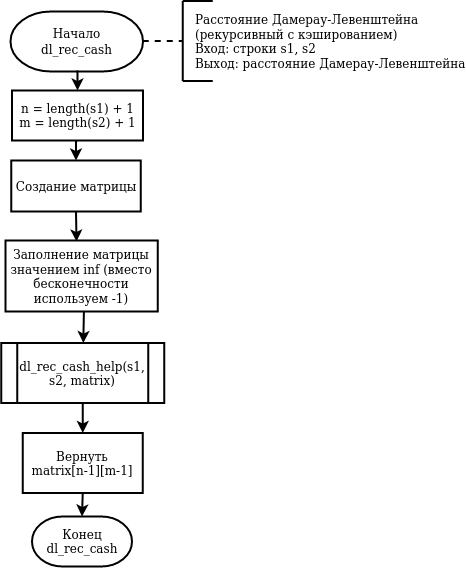
\includegraphics[scale=0.9]{inc/dleven_rec_cash1v2.png}}
		
		\caption{Схема рекурсивного алгоритма поиска расстояния Дамерау-Левенштейна с кешированием}
		
		\label{fig:dleven_rec_cash1}
		
	\end{figure}



\begin{figure}[h!]
	
	\centering{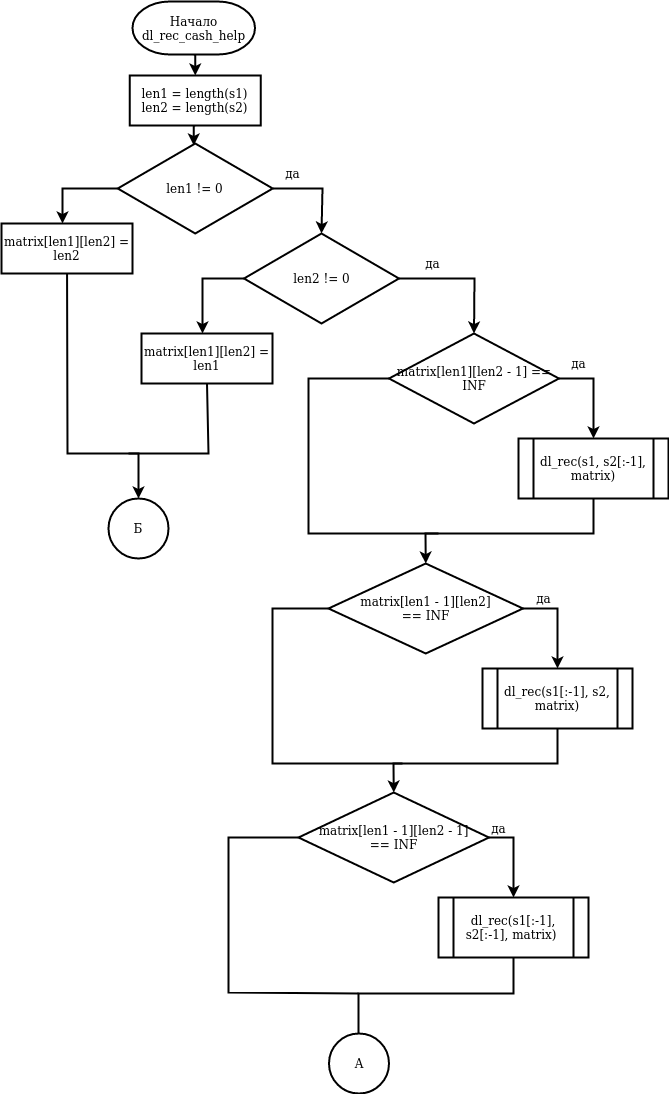
\includegraphics[scale=0.6]{inc/dleven_rec_cash2v2.png}}
		
		\caption{Схема рекурсивного алгоритма поиска расстояния Дамерау-Левенштейна с кешированием}
		
		\label{fig:dleven_rec_cash2}
		
	\end{figure}

\begin{figure}[h!]
	
	\centering{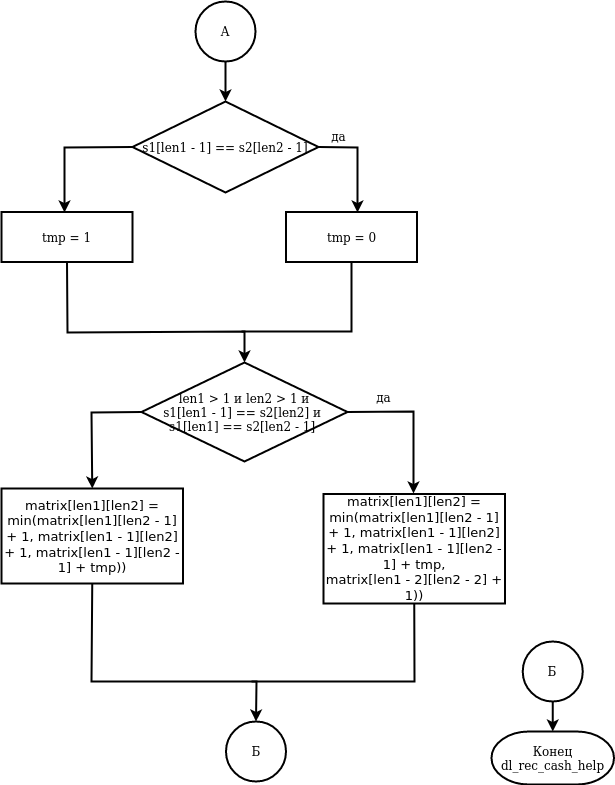
\includegraphics[scale=0.7]{inc/dleven_rec_cash3v2.png}}
		
		\caption{Схема рекурсивного алгоритма поиска расстояния Дамерау-Левенштейна с кешированием}
		
		\label{fig:dleven_rec_cash3}
		
	\end{figure}

\FloatBarrier
\section*{Вывод}


В данном разделе были разработаны схемы алгоритмов, которые позволяютс помощью различных подходов находить расстояния Левенштейна и Дамерау-Левенштейна.

